\documentclass[sigconf]{acmart}

% --- Basic packages and style ---
\usepackage[utf8]{inputenc}
\usepackage[T1]{fontenc}
\usepackage[english]{babel}
\usepackage{microtype}
\usepackage{graphicx}
\usepackage{booktabs}
\usepackage{tabularx}
\usepackage{longtable}
\usepackage{amsmath,amssymb}
\usepackage{siunitx}
\usepackage{caption}
\usepackage{subcaption}
\usepackage{tikz}
\usepackage{pgfplots}
\pgfplotsset{compat=1.18}
\usepackage{enumitem}
\usepackage{listings}
\usepackage{xcolor}
\usepackage{framed}
\usepackage{hyperref}
\usepackage{cleveref}
\usepackage{filecontents}

% --- Colors and listings configuration ---
\definecolor{codebg}{HTML}{F7F7F7}
\definecolor{keyword}{HTML}{0070C0}
\definecolor{comment}{HTML}{008000}
\definecolor{string}{HTML}{A31515}

\lstdefinelanguage{Rust}{
  morekeywords={fn,let,mut,struct,enum,impl,for,while,loop,match,if,else,return},
  sensitive=true,
  morecomment=[l]{//},
  morestring=[b]"
}
\lstset{
  backgroundcolor=\color{codebg},
  frame=single,
  basicstyle=\ttfamily\small,
  keywordstyle=\color{keyword}\bfseries,
  commentstyle=\color{comment}\itshape,
  stringstyle=\color{string},
  breaklines=true,
  showstringspaces=false,
  numbers=left,
  numberstyle=\tiny,
  xleftmargin=6pt, xrightmargin=6pt
}

% --- Metadata (example) ---
\title{Paper Title: A Rich Template with Examples (Lorem ipsum)}
\author{Example Author}
\affiliation{
  \institution{Example University}
  \city{Bogotá}
  \country{Colombia}
}
\date{November 18, 2025}

\begin{document}
\begin{abstract}
Lorem ipsum dolor sit amet, consectetur adipiscing elit. Integer nec odio. Praesent libero. Sed cursus ante dapibus diam. This document is a neutral-English template showcasing figures, equations, tables, code, and appendices.
\end{abstract}

\maketitle

\section{Introduction}
Lorem ipsum dolor sit amet, consectetur adipiscing elit. Vestibulum \emph{vulputate} diam sit amet nulla accumsan, ut ultricies mi faucibus.\footnote{Example footnote illustrating footnote usage.} See Section~\ref{sec:methods} for methodology details.

% --- Equations (inline and display) ---
Text with an inline equation \(E = mc^2\) and a displayed equation:
\begin{equation}
\label{eq:quadratic}
f(x) = a x^2 + b x + c
\end{equation}
Multiple aligned equations:
\begin{align}
\label{eq:system}
y &= m x + b, \nonumber\\
z &= \sin(\theta) + \cos(\theta).
\end{align}

\section{Methods}
\label{sec:methods}
Lorem ipsum dolor sit amet, consectetur adipiscing elit. Below are lists and structural examples.

\subsection{Lists}
\begin{itemize}[leftmargin=*]
  \item Simple bullet item with lorem ipsum filler.
  \item Item with a nested enumerated list:
    \begin{enumerate}
      \item First step.
      \item Second step.
    \end{enumerate}
  \item Description list:
    \begin{description}
      \item[Dataset] Simulated dataset used for demonstration.
      \item[Metric] \(\mathrm{RMSE} = \sqrt{\frac{1}{n}\sum_{i=1}^n (y_i - \hat{y}_i)^2}\).
    \end{description}
\end{itemize}

% --- Tables: several types ---
\subsection{Tables: multiple examples}
\paragraph{Simple table using booktabs}
\begin{table}[ht]
  \centering
  \caption{Simple summary table (booktabs).}
  \label{tab:simple}
  \begin{tabular}{lrr}
    \toprule
    Group & Mean & Std. Dev. \\
    \midrule
    A & 12.3 & 1.4 \\
    B & 10.8 & 2.1 \\
    C & 14.0 & 0.9 \\
    \bottomrule
  \end{tabular}
\end{table}

\paragraph{Tabularx for wide descriptive columns}
\begin{table}[ht]
  \centering
  \caption{Wide table with automatic wrapping.}
  \begin{tabularx}{\linewidth}{@{}lXc@{}}
    \toprule
    Variable & Description & Value \\
    \midrule
    $x$ & Lorem ipsum dolor sit amet, consectetur adipiscing elit, sed do eiusmod tempor. & 3.14 \\
    $y$ & Another long description that wraps automatically within the cell. & 2.71 \\
    \bottomrule
  \end{tabularx}
\end{table}

\paragraph{Longtable (multi-page) example}
\begin{longtable}{lll}
  \caption{Example longtable (may span pages).} \\
  \toprule
  ID & Name & Note \\
  \midrule
  \endfirsthead
  \multicolumn{3}{c}{\textit{Continued from previous page}} \\
  \toprule
  ID & Name & Note \\
  \midrule
  \endhead
  \midrule \multicolumn{3}{r}{\textit{Continued on next page}} \\
  \endfoot
  \bottomrule
  \endlastfoot
  1 & Alpha & lorem ipsum \\
  2 & Beta & dolor sit \\
  3 & Gamma & amet \\
  % More rows can follow...
\end{longtable}

% --- Figures and subfigures ---
\section{Figures}
\label{sec:figures}
Lorem ipsum dolor sit amet. The example below shows subfigures and a pgfplots chart.

\begin{figure}[ht]
  \centering
  \begin{subfigure}[b]{0.45\linewidth}
    \centering
    % Replace with your file path: images/placeholder1.png
    \includegraphics[width=\linewidth]{images/placeholder1.png}
    \caption{Subfigure A (PNG).}
    \label{fig:subA}
  \end{subfigure}\hfill
  \begin{subfigure}[b]{0.45\linewidth}
    \centering
    % Replace with your file path: images/placeholder2.pdf
    \includegraphics[width=\linewidth]{images/placeholder2.pdf}
    \caption{Subfigure B (PDF).}
    \label{fig:subB}
  \end{subfigure}
  \caption{Example of subfigures.}
  \label{fig:subfigs}
\end{figure}

\paragraph{Advanced figure: plot with pgfplots}
\begin{figure}[ht]
  \centering
  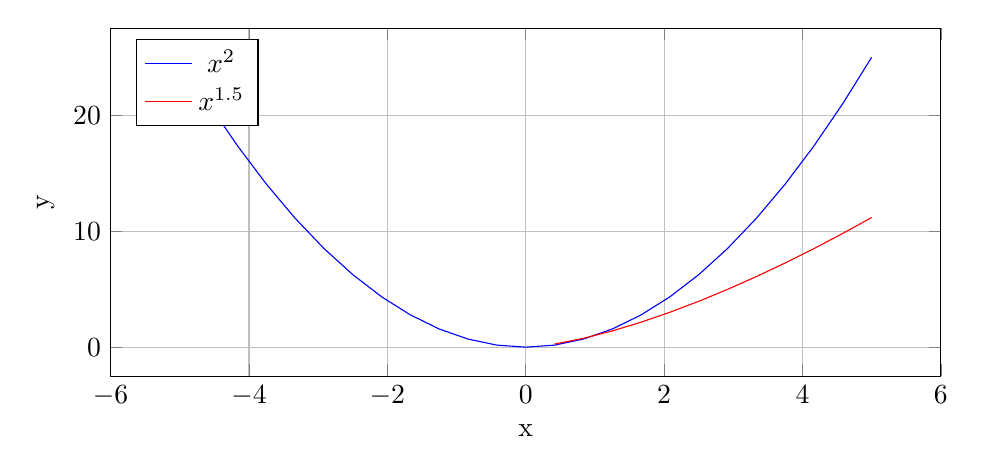
\begin{tikzpicture}
    \begin{axis}[
      width=\linewidth,
      height=6cm,
      xlabel={x},
      ylabel={y},
      grid=both,
      legend pos=north west
    ]
      \addplot+[mark=none] {x^2};
      \addplot+[mark=none] {x^1.5};
      \legend{$x^2$,$x^{1.5}$}
    \end{axis}
  \end{tikzpicture}
  \caption{Example plot generated with \texttt{pgfplots}.}
  \label{fig:pgfplot}
\end{figure}

% --- TikZ diagram / flowchart ---
\subsection{Diagram / Flowchart (TikZ)}
\begin{figure}[ht]
  \centering
  \begin{tikzpicture}[node distance=12mm, auto, every node/.style={draw,rounded corners,fill=white}]
    \node (start) {Start};
    \node (upload) [below=of start] {Upload code / problem};
    \node (gen) [below=of upload] {Generate questions (LLM)};
    \node (rev) [below=of gen] {Review / Filter};
    \node (out) [below=of rev] {Output: questions \& feedback};
    \draw[->] (start) -- (upload) -- (gen) -- (rev) -- (out);
  \end{tikzpicture}
  \caption{High-level flowchart (TikZ).}
  \label{fig:flow}
\end{figure}

% --- Code examples: Python, C++, Rust ---
\section{Code Examples}
\subsection{Python}
\begin{lstlisting}[language=Python,caption={Python example: simple solution},label={lst:py}]
def fibonacci(n):
    """Return the Fibonacci sequence up to n elements."""
    a, b = 0, 1
    res = []
    for _ in range(n):
        res.append(a)
        a, b = b, a + b
    return res
\end{lstlisting}

\subsection{C++}
\begin{lstlisting}[language=C++,caption={C++ example: sum},label={lst:cpp}]
#include <bits/stdc++.h>
using namespace std;
int main(){
    ios::sync_with_stdio(false);
    cin.tie(nullptr);
    int n; cin >> n;
    long long sum = 0;
    for(int i=0;i<n;i++){ int x; cin>>x; sum += x; }
    cout << sum << "\n";
    return 0;
}
\end{lstlisting}

\subsection{Rust}
\begin{lstlisting}[language=Rust,caption={Rust example: read and parse},label={lst:rust}]
fn main() {
    use std::io::{self, Read};
    let mut s = String::new();
    io::stdin().read_to_string(&mut s).unwrap();
    println!("Input length: {}", s.len());
}
\end{lstlisting}

% --- Results: statistical tables and commentary ---
\section{Results}
Lorem ipsum dolor sit amet, consectetur adipiscing elit. Table~\ref{tab:stats} summarizes descriptive statistics.

\begin{table}[ht]
  \centering
  \caption{Descriptive statistics (simulated).}
  \label{tab:stats}
  \begin{tabular}{lrrrr}
    \toprule
    Group & $n$ & Mean & Median & Std. Dev. \\
    \midrule
    Control & 50 & 12.34 & 12.0 & 2.1 \\
    Treatment & 48 & 13.85 & 13.5 & 1.8 \\
    \bottomrule
  \end{tabular}
\end{table}

We note non-linear trends in the experiment (see Figure~\ref{fig:pgfplot}).

% --- Discussion and conclusion ---
\section{Discussion}
Lorem ipsum dolor sit amet, consectetur adipiscing elit. See Equation~\eqref{eq:quadratic} for the proposed model.

\section{Conclusion}
Lorem ipsum dolor sit amet. Future work includes integrating retrieval-augmented methods and improving the interactive GUI.\footnote{Additional note on future improvements.}

\section*{Acknowledgments}
We thank \ldots (Lorem ipsum).

% --- Bibliography: embedded references.bib for convenience ---
\begin{filecontents}{references.bib}
@article{knuth84,
  author = {Knuth, Donald E.},
  title = {Literate Programming},
  journal = {The Computer Journal},
  year = {1984},
  volume = {27},
  number = {2},
  pages = {97--111}
}
@inproceedings{doe2021,
  author={Doe, John and Roe, Jane},
  title={Automatic Generation of Programming Exercises Using LLMs},
  booktitle={Proceedings of the Example Conference},
  year={2021},
  pages={123--130},
  publisher={IEEE}
}
@article{smith2019,
  author = {Smith, A. and Example, B.},
  title = {A Survey on Educational Tools},
  journal = {IEEE Trans. on Education},
  year = {2019},
  volume = {62},
  number = {4},
  pages = {345--359}
}
\end{filecontents}

\bibliographystyle{IEEEtran}
\bibliography{references}

% --- Appendices ---
\appendix
\section{Appendix A: Additional Material}
Lorem ipsum dolor sit amet, additional appendix material.

\section{Appendix B: Utility code}
\begin{framed}
\textbf{Note}: For long code listings consider including external files and referencing them.
\end{framed}

\end{document}
